%% Autor: Björn Ritterbecks 
%% Letzte Aenderung: 15.06.2016 
\thisfloatsetup{%
  capbesidewidth=\marginparwidth}
\begin{figure}[htbp]
\vspace*{0.2cm}
\centering
%\sansmath
 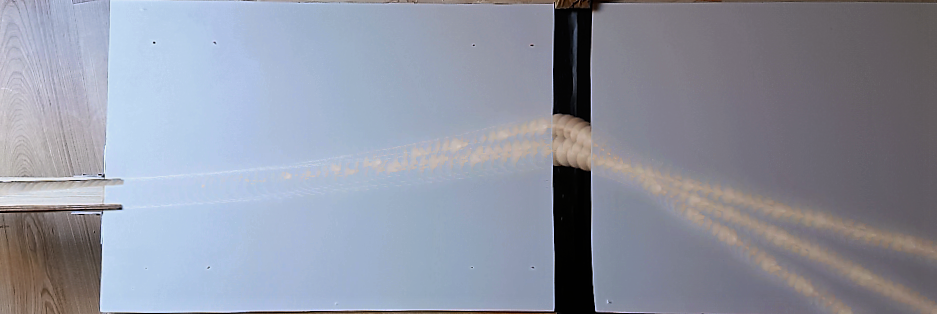
\includegraphics[width=0.99\textwidth]{images/aufbau2.png}
  \caption[Stroboskop-Effekt der Kugeln 8--10]{Die Bahnen der Kugeln 8--10 der Messreihe mit Kugeldurchmesser $r=\SI{35}{\milli\metre}$. Die Rampe befindet sich bei $y=\SI{0}{\centi\metre}$, die Düse des Gebläses bei $x=\SI{60}{\centi\metre}$ und $y=\SI{25}{\centi\metre}$.}
  \label{fig:aufbau2}
  \vspace{-0pt}
\end{figure}